\chapter{Introduction}\label{ch:BPixIntro}

The extremely high particle fluxes at small distances from the interaction point require the innermost tracking layers to be composed of pixel devices delivering spatial information with high resolution.
Over the full acceptance of the CMS detector, the silicon pixel system provides two or more hits per track, which allow secondary vertices to be reconstructed for tagging long-lived objects, like b or c quarks and $\tau$-leptons, and to distinguish them from a large background of light quark and gluon jets. It is also an important detector for identifying the primary vertex, and separating it from dozens of additional pileup vertices.
Hence, this detector plays a special role in the physics analyses described in this thesis. In fact, its performance has a large impact on the identification of b-quark jets as well as on jet substructure observables, being the latter highly dependent on pileup.
%The CMS pixel detector allows for high precision tracking in the region closest to the inter- action point in a particularly harsh environment characterized by a high track multiplicity and heavy irradiation. The main purpose of the pixel detector is the reconstruction of secondary vertices from heavy flavor and tau decays and the generation of track seeds for track reconstruction.
The pixel detector consists of central barrel layers (BPix) and forward disks (FPix).
This part of the thesis is dedicated to different aspects of the BPix system, including its calibration and upgrade.\\ 

%LHC started in 2008 and it is expected to be operative up to the 2035 (Fig.~\ref{fig:LHCplan}).
The pixel detector was installed in 2008 and showed an excellent performance during the first period of data taking at the LHC (2010--2012).
During the first long shut-down of the machine (2012--2015), that allowed to increase the center-of-mass energy of the collisions to 13\TeV, the detector was extracted for repair and re-installed into CMS, and successfully continued taking data throughout the first two years of LHC Run~2 (2015--2016). The excellent performance of the BPix at the re-start of collisions have been made possible by the efforts spent during LS1 in recovering the broken channels as well as in re-calibrating the detector after the radiation damage suffered during Run~1.

The current planning for the LHC and injector chain foresees other two long shut-downs, LS2 and LS3 (Fig.~\ref{fig:LHCplan}).
In the period through LS2 (2019--2020), the injector chain will be improved,
and during LS3 (2024--2026) the LHC itself will be upgraded with new components to optimize the bunch overlap at the interaction region. 
Further upgrades are foreseen beyond 2030.

The present pixel detector was originally designed for a luminosity of $1\times10^{34}\percms$ and a pileup of 25 in LHC collisions with 25\unit{ns} bunch spacing.
These parameters have already been exceeded in 2016, when collisions at 13\TeV happened at instantaneous luminosities up to $1.5\times10^{34}\percms$ with an average pileup of 25~\cite{LumiPublicResults}.
Based on the excellent LHC performances to date, it can be anticipated that the peak luminosity will keep increasing until 2018 reaching values up to 1.7--1.8$\times10^{34}\percms$, and beyond these after LS2.
Thus, starting from 2017 the CMS experiment must be prepared to operate with an average pileup of 50 as a baseline,
with the possibility that it may be significantly higher (up to 100) if collisions will happen at 50\unit{ns} bunch spacing after LS2.
In order to maintain efficient and robust tracking at CMS, the pixel detector will be replaced with an upgraded pixel system, referred to as {\it Phase~1 pixel upgrade}, in the LHC winter shutdown 2016/2017.
The design of the upgraded detector allows to cope with the aforementioned harsh conditions expected at the LHC in the upcoming years.
A more complex upgrade step is planned for the LS3 and referred to as {\it Phase~2 upgrade}. It will include deeper changes in the whole CMS, among which a complete substitution of the entire tracker detector system.

The Phase~1 pixel detector is expected to be operative up to the Phase~2 upgrade, around 2023.
During the planned 5 years of operation before LS3, the LHC is expected to deliver about 500\fbinv.
%Particle fluence has been estimated based on pixel cluster counting in the present detector and the expected absorbed ionizing dose for the different tracker detectors is reported in Fig. 2.2.
The proposed Phase~1 upgrade system has been designed and tested to be operative up to this target, with the only exception of the innermost layer.
In fact, the estimated hadron fluence that will be accumulated in the innermost pixel layer is too high for the pixel sensor, thus a replacement of the innermost barrel layer is planned after 250\fbinv.
%The hadron fluence that will be accumulated in the innermost pixel layer at $r = 3\cm$ for 500\fbinv is estimated to be $F = 3.0\times10^{15}n_{eq}cm^{?2}$.
%This value is too high for the pixel sensor, thus a replacement of the innermost barrel layer is planned after 250\fbinv.

The Phase 1 pixel upgrade project is now at its last stage of assembly and testing of the entire system.
A test stand has been setup at the University of Zurich (UZH) in 2014 and was operated until the end of 2016. It has been fundamental to test the performance of the complete upgraded BPix system and gain experience in its operation.
This activity is crucial in view of the success of the installation and commissioning of the new detector planned for the beginning of March 2017, as well as for excellent and stable performance during its first year of data-taking.\\

This part of the thesis is organized as follows.
First, a description of the design and functionality of the present BPix detector is given in Chapter~\ref{ch:BPix}.
The work carried out during LS1 aimed at optimizing the detector for LHC Run~2 is discussed in Chapter~\ref{ch:BPixCalib}.
The same chapter also includes details on the operations conducted during its re-installation into CMS and commissioning.
Chapter~\ref{ch:Phase1Intro} provides an overview of the design and features of the upgraded BPix system.
In this chapter, a section is dedicated to the description of the test stand at UZH which I contributed to setup.
The last section focuses on the development of new tests and procedures to be used during the upgraded detector assembly and commissioning.

\begin{figure}[!t]
 \begin{center}
 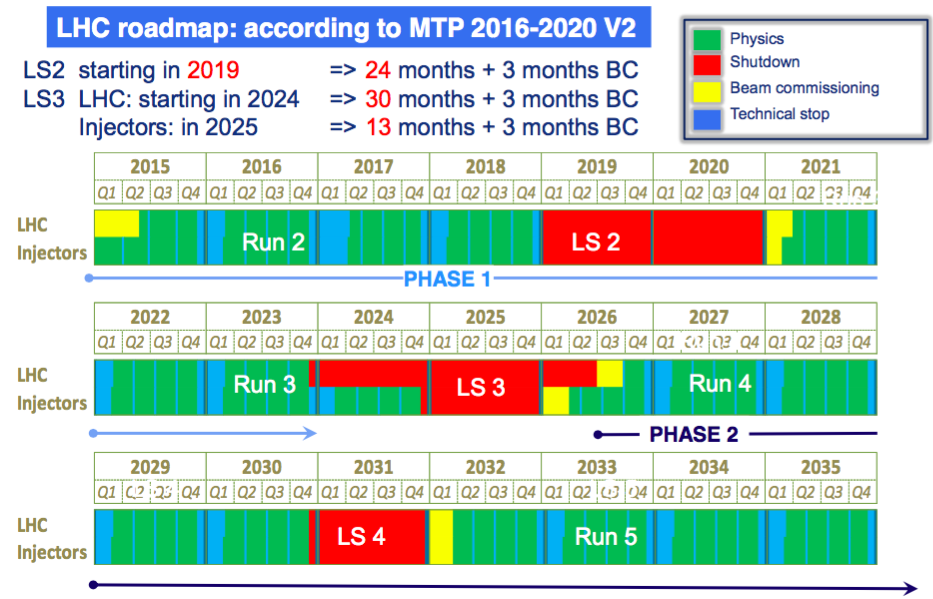
\includegraphics[width=0.8\textwidth]{\chthirteen/LHCplan-approved.png}
 \end{center}
 \caption{The outline LHC schedule up to 2035 as officially approved in June 2015~\cite{LHCpage}.}
 \label{fig:LHCplan}
\end{figure}